\documentclass[a4paper,10pt,twoside,twocolumn]{dndbook} %a4, 10pt, book (idk why i did that...), 2 cols, dnd-themed
\usepackage[english]{babel} %language
\usepackage[utf8]{inputenc} %lovely utf-8
\usepackage{graphicx} %images
\usepackage{wrapfig} %images
\usepackage{array} %allways use this shit, idk why
\usepackage{tikz} %draw stuff
\usepackage{ifthen} %draw stuff
\usetikzlibrary{shapes,calc,fadings} %draw stuff
\usepackage{xspace} %usefull idk, allways import this stuff
\usepackage{dirtytalk} %\say because fuck it
\usepackage{setspace} %don't ask, kind of like it...
\usepackage{pgfplots}

\usepackage[singlelinecheck=false]{caption} %idk dndbook...
\usepackage{listings} %idk dndbook...
\usepackage{shortvrb} %not used yet...
\usepackage{stfloats} %idk dndbook
\usepackage{dirtytalk}

\singlespacing
\makeatletter %because of titlepage and \HUGE

\@openrightfalse %no empty pages

\graphicspath{ {./images/} }

\def \license {GNU Free Documentation License}
\def \licensetext {Please consider and respect the copyleft of this license. The content of this document should be accessible to everyone. Everyone has the right to use the content of this document as he/she wishes, to modify it, to publish it modified (taking into account the copyleft) and to republish it without any changes (taking into account the copyleft).}
\def \author {Sven Hugi}%if you edit this document, add your name... <3
\def \illustrators {} %add name
\def \othercontrib {} %add name

%highlighting with some random effect -> looks handmade and i love it...
\newcommand\hl[2][yellow]{
	\begin{tikzpicture}[
	baseline,
	decoration={random steps,amplitude=1pt,segment length=15pt},
	outer sep=-15pt, inner sep = 0pt
	]
	\node[decorate,rectangle,fill=#1,anchor=text]{#2\xspace};
	\end{tikzpicture}
}
%2 column layout hack...
\newcommand{\nextPage}{
	\newpage
	\hbox{}
	\newpage
}
%make bad things look ok...
\newcommand{\doublelinebreak}{
	\linebreak\linebreak
}
%the old HUGE fontsize
\newcommand\HUGE{\@setfontsize\Huge{60}{80}} 

\renewcommand{\maketitle}{
	\thispagestyle{empty}
	\onecolumn %fuck it
	\vspace*{5cm}
	\begin{center}
		$\vspace*{2cm}$
			{\HUGE\DndFontDropCap{WIGHT}}\\	
	\end{center}
	\twocolumn %reset shit
}\makeatother

\begin{document}
	\maketitle
	\section*{Credits}
	\vspace{.25cm}
	\textbf{Authors:} \author\linebreak
	\textbf{Illustrators:} \illustrators\linebreak
	\textbf{Additional Contributors:} \othercontrib\linebreak
	\textbf{License:} \license\doublelinebreak
	\licensetext\doublelinebreak
	Inspiration from the Monster Manual\linebreak
	Images and Flavourtext from fandom.com
	\vfill\pagebreak\hbox{}\vfill\hfill{\tiny This Document was written in \LaTeX.}\pagebreak\vfill\pagebreak
	\DndDropCapLine{W}{}ights appeared as weird and twisted reflections of the forms they had in life. They existed in a state between being alive and being dead. When attacking their prey, wights' eyes glowed like white-hot embers. Their mummified flesh covered the twisted skeleton, the hands ended up in deadly claws, and teeth were sharp and jagged like needles.\linebreak
	Wights were evil undead creatures brought back to unlife by their vanity, evil deeds, and desires. Upon the ends of their mortal lives, the dying spirits reached out to Orcus or another evil deity, receiving undeath in exchange for spending eternity, hating and trying to destroy all living beings.\linebreak
	Wights retained their personalities and memories in the undeath. They possessed free will at the same time as they were tasked to perform the bidding of the evil powers that brought them back.\linebreak
	Even though wights hungered for living beings' energy, they did not require it as a source of sustenance. The wights could retain their undeath trapped in tombs for centuries. Their craving for life energy was more akin to an addiction. Sages theorized that when a wight drained a victim's life energy, it received a rush of mortality, euphoric reminder of their mortal existence. Chasing that feeling led to extremely depraved actions by wights.\linebreak
	Wights were active at night, retreating away from the hated sunlight into crypts, tombs, burial mounds, where they dwelt during the day. Unlike vampires though, wights simply disliked the sun, not harmed by it.
	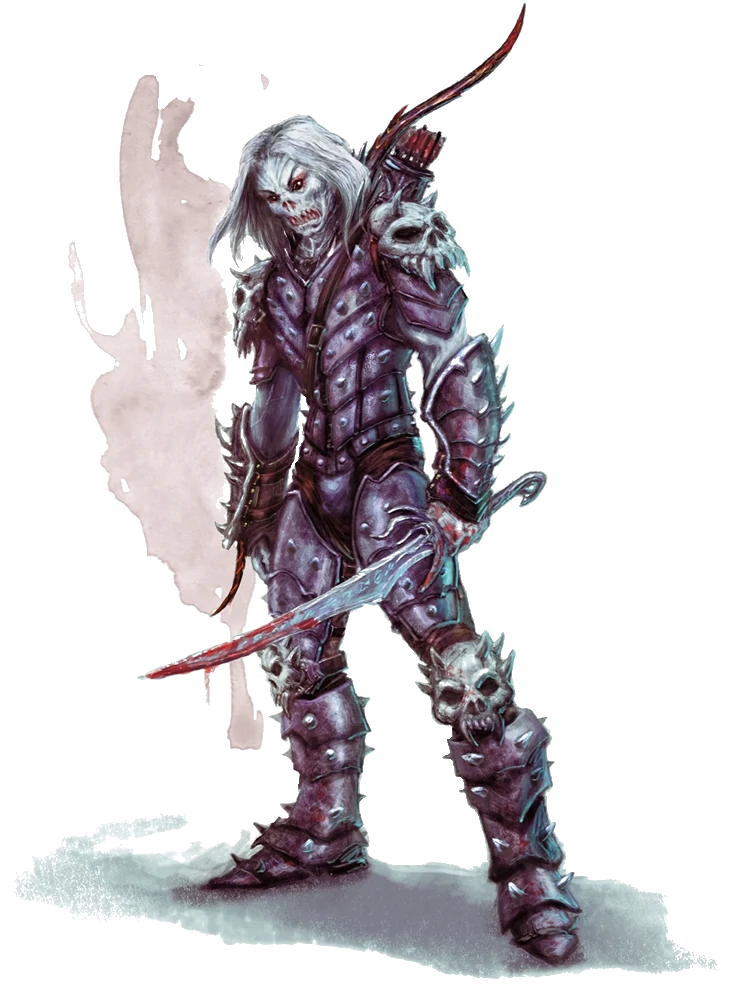
\includegraphics[width=\linewidth]{Wight.png}
	\vfill\pagebreak
	\section{Wight Traits}
	\textbf{Ability Score Increase.} Your Charisma score increases by 2 and your Constitution score increases by 1.\linebreak
	\textbf{Age.} Wights do not age after death.\linebreak
	\textbf{Alignment.} Any Evil\linebreak
	\textbf{Size.} Wight's stand between 5 and 6 feet tall and average about 120 pounds. Your size is Medium.\linebreak
	\textbf{Speed.} Your base walking speed is 30ft.\linebreak
	\textbf{Language.} Choose any 2.\linebreak
	\textbf{Damage Resistances.} Necrotic, Poison\linebreak
	\textbf{Vulnerability.} Holy Wather, Radiant Damage\linebreak
	\textbf{Undead Nature.} You are considered of the undead type. You doesn't require air, food, drink or sleep. But you can not be healt by any sort of healing magic, instead you take damage. \linebreak
	\textbf{Superior Darkvision.} You can see in dim light within 120 ft of you as if it were bright light, and in darkness as if it were dim light. You can't discern color in darkness, only shades of gray.\linebreak
	\textbf{Nightmare.} You can't sleep. Also magic can't put you to sleep. 4 hour of light activity count for you as longrest.\linebreak
	\textbf{Sunlight Sensitivity.} While in sunlight, you have disadvantage on attack rolls, as well as on Wisdom (Perception) checks that rely on sight.\linebreak
	\textbf{Necromantic Regeneration.} If you reduce the hit points of a creature with a melee weapon attack or necromantic damage to 0 you regain hit points equal to your proficiency bonus. If the creature has more max hit points thay you, you can add your level to the regain hit points. You can also leech hit points from a willing, living, non-construct creature.\linebreak
	\subsection{Subrace} The subrace determines what you were before you died. Choose from:\linebreak
	\subsubsection{Human}
	\textbf{Proficiency.} You gain proficiency in one skill of your choice.
	\subsubsection{High Elf}
	\textbf{Cantrip.} You know one cantrip from the wizard spell list. Intelligence is your spellcasting ability for it.
	\subsubsection{Wood Elf}
	\textbf{Keen Sense.} You gain proficiency in the Perception skill.
	\subsubsection{Dark Elf}
	\textbf{Drown Weapon Training.} You gain proficiency with Rapier, Shortsword and Hand Crossbow.
	\subsubsection{Sea Elf}
	\textbf{Swimm Speed.} You have a swimming speed of 30 feet.
	\subsubsection{Halfling}
	\textbf{Nimbleness.} You can move throught the space of any creature that is of a size larger than yours.\linebreak
	\textbf{Size.} Your size is Small.
	\subsubsection{Hill Dwarf}
	\textbf{Dwarfen Toughness.} Your hit point maximum is increased by 1 for every level.
	\subsubsection{Mountain Dwarf}
	\textbf{Dwarfen Armor Training.} You gain proficiency with light and medium armor.
	\subsubsection{Gnome}
	\textbf{Gnome Cunning.} You have advantage on all Intelligence, Wisdom and Charisma saving throws against magic.\linebreak
	\textbf{Size.} Your size is Small.
	\subsubsection{Half Orc}
	\textbf{Meancing.} You gain proficiency in the Intimidation skill.
	\subsubsection{Orc}
	\textbf{Powerful Build.} You count as one size larger when determining your carrying capacity and the weight you can push, drag, or lift.
	\subsubsection{Tiefling}
	\textbf{Hellish Resistance} You have resistance to fire damage.
	\subsubsection{Dragonborn}
	\textbf{Breath Weapon.} You can use your action to exhale destructive energy. It deals acid damage in a 15ft cone. When you use your breath weapon, all creatures in the area must make a dexterity saving throw. The DC of this saving throw is 8 + your Constitution modifier + your proficiency bonus. A creature takes 2d6 damage on a failed save, and half as much damage on a successful one. The damage increase to 3d6 at 6th level, 4d6 at 11th, and 5d6 at 16th level. After using your breath weapon, you cannot use it again until you complete a short or long rest.
	\subsubsection{Tabaxi}
	\textbf{Cat's Claws.} Because of your claws, you have a climbing speed of 20 feet. In addition, your claws are natural weapons, which you can use to make unarmed strikes. If you hit with them, you deal slashing damage equal to 1d4 + your Strength modifier.
	\subsubsection{Kenku}
	\textbf{Mimicry.} You can mimic sounds you have heard, including voices. A creature that hears the sounds you make can tell they are imitations with a successful Wisdom (Insight) check opposed by your Charisma (Deception) check.\linebreak
	\textbf{Can't Speek.} You can speak only by using your Mimicry trait.
	\subsubsection{Kobold}
	\textbf{Pack Tactics.} You have advantage on an attack roll against a creature if at least one of your allies is within 5 feet of the creature and the ally isn't incapacitated.\linebreak
	\textbf{Size.} Your size is Small.
	\subsubsection{Goblin}
	\textbf{Nimble Escape.} You can take the Disengage or Hide action as a bonus action on each of your turns.\linebreak
	\textbf{Size.} Your size is Small.
	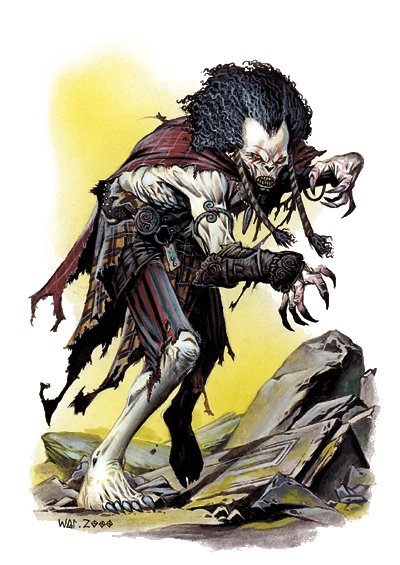
\includegraphics[width=\linewidth]{Wight2.png}
	
\end{document}